% \documentclass[a4paper,twocolumn,10pt]{article}
\documentclass[conference]{IEEEtran}
\IEEEoverridecommandlockouts
\usepackage{fontspec}
\usepackage{biblatex}
\usepackage{graphicx}
\usepackage{amsmath}
\usepackage{subfig}
\usepackage{algorithm2e}
\bibliography{report.bib}
\defaultfontfeatures{Mapping=tex-text}
\setromanfont[Ligatures={Common},Numbers={Lining}]{Linux Libertine}

\title{Multi-object Tracking of Vehicles using Kalman and Particle Filters}
\author{Michal Staniaszek \thanks{Project completed with Carlos G\'{a}lvez Del Postigo.}}

\begin{document}
\maketitle

\begin{abstract}
  In this report, we detail a system capable of simultaneously tracking multiple
  vehicles in a highway scene, from a fixed camera above the road. We use a
  mixture of Gaussians to segment the scene into foreground and background
  pixels. Blob detection is used to extract the bounding box and centroid of the
  blobs, which are then passed to a filter. We present two methods of tracking
  --- multiple Kalman filters, or a modified particle filter. The filters are
  able to process video at a rate of 5 and 2 frames per second respectively,
  with good results when the environment is uncomplicated. Performance degrades
  in night scenes, and when occlusions occur.
\end{abstract}


\section{Introduction}
The tracking of vehicles is an active area of research. Over the past two
decades, a large number of different techniques have been developed or employed
for the purpose of vehicle tracking. Broadly speaking, there are two different
scenarios which are often encountered. First, we have the case in which the
camera is mounted on a moving vehicle, and we attempt to track the motion of
target vehicles, in order to assist the driver, or to give as input to an
autonomous driving system. The other case is that in which we have a fixed
camera looking at a portion of road, and we wish to track the vehicles entering
and exiting the field of view of the camera, also known as traffic
surveillance. Previous research in traffic surveillance deals with tracking and
classification \cite{hsieh2006automatic,meier1999tracking}, and traffic flow and
vehicle speed calculation \cite{hsu2004real,coifman1998real}. Numerous methods
are used in order to extract the relevant data. For example, lane-dividing lines
can be used to eliminate problems relating to shadows \cite{hsieh2006automatic},
and using a-priori road information to improve the tracking quality
\cite{magee2004tracking}. In order to extract information from the image, some
visual processing is required. There are several methods that have been used to
extract vehicles from images, including 3D detection and description
\cite{kim2003fast}, Gaussian mixture models for background and foreground
extraction \cite{stauffer1999adaptive}, and methods using optical flow
\cite{javed2006tracking}.

Systems which extract and process this information can be used in intelligent
transport systems in order to monitor traffic conditions and attempt to reduce
congestion. The simplest useful system is one which tracks the position and
velocity of vehicles in the image, and we will discuss our implementation of
such a system in the subsequent sections.
\section{Object Extraction}
\subsection{Mixture of Gaussians}
The first step after obtaining a video to process is to extract the objects of
interest in the image. Our approach uses Gaussian mixture models technique
developed by Stauffer~\cite{stauffer1999adaptive}. This technique allows the
separation of background pixels and foreground pixels by using multiple
Gaussians. Each pixel is represented by some $K$ Gaussians, and the persistence
and variance of these are used to determine whether a certain pixel is a
background or foreground pixel in any given image of the sequence. As each pixel
can have multiple surfaces present within it, and the illumination can also
change, multiple Gaussians are required to fully represent the possible range of
background pixel values. We make the assumption that Gaussian noise is added to
the value of the pixel which is measured by the sensor, either due to random
noise, or due to small fluctuations in the illumination. For each pixel in the
image, the probability of observing its current value is~\cite{stauffer1999adaptive}
\begin{equation}
  P(X_t)=\sum_{i=1}^Kw_{i,t}\cdot\eta(X_t,\mu_{i,t},\Sigma_{i,t})
\end{equation}
where $X_t$ is the pixel value, $\mu_{i,t}$ and $\Sigma_{i,t}$ are the mean and
covariance of the $i$th Gaussian at time $t$, $\eta$ represents the normal
distribution. $w_{i,t}$ is a weight assigned to each Gaussian which estimates
how much of the data that has been seen so far is accounted for by this
Gaussian. Since we are dealing with colour images, the Gaussians are
multivariate, but we make the assumption that each colour is independent and has
the same variance, and therefore the covariance for each Gaussian is
\begin{equation}
  \Sigma_{k,t}= \sigma_k^2\mathbf{I}
\end{equation}

At each timestep, the Gaussian closest to the current pixel value is
computed. If it is within 2.5 standard deviations (computed using the
Mahalanobis distance), then we update the mean and covariance of the matched
Gaussian as follows
\begin{align}
  \mu_t&=(1-\rho)\mu_{t-1}+\rho X_t\\
  \sigma_t^2&=(1-\rho)\sigma_{t-1}^2+\rho(X_t-\mu)^T(X_t-\mu)
\end{align}
where $\rho$ is a learning rate
\begin{equation}
  \rho=\alpha\eta(X_t\mid \mu_k,\sigma_k)
\end{equation}
The parameters of other Gaussians are not updated, but their weight is updated
according to
\begin{equation}
  w_{k,t}=(1-\alpha)w_{k,t-1}+\alpha(M_{k,t})
\end{equation}
where $\alpha$ is another learning rate, which ``describes an exponentially
decaying envelope that is used to limit the influence of old
data''~\cite{zivkovic2004improved}. We set $\alpha$ to 0.01. The weights are
normalised after this operation. If it is the case that none of the current
distributions matches the pixel, then the one with the lowest probability is
replaced with a Gaussian with a mean corresponding to the current pixel value, a
high variance, and a low weight.

To estimate the background model, we need to find which of the Gaussians in the
model are most likely to represent background pixels, heuristically those with
the lowest variance, and most supporting evidence
\cite{stauffer1999adaptive}. When some object is static, the variance in its
pixels is very low, generally coming only from noise. This results in the
Gaussians building up a large body of evidence to suggest that this is a
background pixel, represented by their weights. When a moving object comes into
the scene and occludes the background, it will either be attached to one of the
existing Gaussians, increasing its variance, or it will be too dissimilar and
therefore a new distribution will be created to account for it. To deal with
these issues, we choose some part of the mixture model to represent the
background; the rest will represent dynamic objects in the image. Gaussians are
ordered according to the value $w/\sigma$, a value that increases the lower the
variance, and the more supporting evidence the Gaussian has. The background
model is chosen as
\begin{equation}
  B = \underset{b}{arg\;min}\left(\sum_{k=1}^bw_k>T\right)
\end{equation}
$T$ defines the proportion of the image that should be considered as background
data. The value $B$ gives the index of the last Gaussian that should be
considered part of the background model --- all subsequent Gaussians are part of
the foreground. The value of $T$ depends on the video that is being
processed. If there are a large number of foreground objects, then its value may
be quite low. In our case, we have found that a value of approximately 0.6 is
appropriate. Using this and the value we choose for $\alpha$, the number of
frames $\tau$ taken for an object to be considered background
is~\cite{zivkovic2004improved}
\begin{equation}
  \tau=\frac{\log(0.6)}{\log(1-0.01)}\approx 51
\end{equation}
\subsection{Morphological Operations and Blob Detection}
Once the foreground pixels have been determined, we perform further processing
to extract objects from the image and transform the pixel data into something
which can be used for tracking. An example of the image received from the
mixture of Gaussians can be seen in Figure~\ref{fig:extracted}. The extracted
foreground pixels do not fully cover the object --- this is likely because some
parts of the vehicles have colours which are similar to the background
pixels. We would like to fill in these holes and receive a uniform blob to work
on. First, we need to apply some morphological operations in order to make the
second stage of the process easier. Morphological operations are ``a tool for
extracting image components that are useful in the representation and
description of region shape'' \cite{gonzalez2008digital}. We are particularly
interested in the operations of erosion, dilation and filling. Erosion is an
operation that shrinks or thins regions in a binary image. This allows us to get
rid of some of the smaller features that might be present in the image that are
not relevant to what we are trying to extract. Dilation is the opposite to
erosion. Instead of shrinking regions, it grows or thickens them. This allows us
to connect regions that were not connected for whatever reason. The filling
operation, as the name suggests, fills holes in an image. The holes must be
surrounded by 8-connected boundaries \cite{gonzalez2008digital}. Two pixels are
8-connected if one can be reached from the other by taking a 1-pixel step in
horizontal or diagonal directions.

The first operation we apply is dilation, in order to bridge gaps
in the vehicles, which are often caused by the windscreen. Then, we fill holes
in the image, which are again usually caused by the windscreen. Finally, to
disconnect regions that should not be connected which may have been connected by
the dilation operation, or to remove noise pixels and other very small regions,
we use erosion. Once these operations have been done, we obtain something which
looks like Figure~\ref{fig:morphed}.

\begin{figure}
  \centering
    \subfloat[]{
      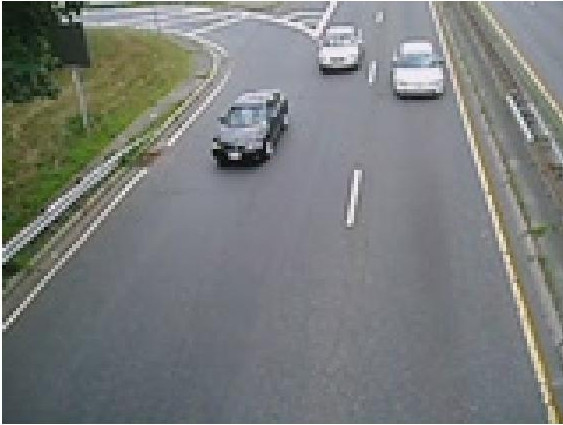
\includegraphics[height=.35\linewidth]{img/original.jpg}
    }
    \subfloat[]{
      \label{fig:extracted}
      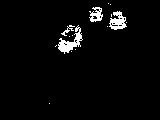
\includegraphics[height=.35\linewidth]{img/fg_extracted.jpg}
    }\\
    \subfloat[]{
      \label{fig:morphed}
      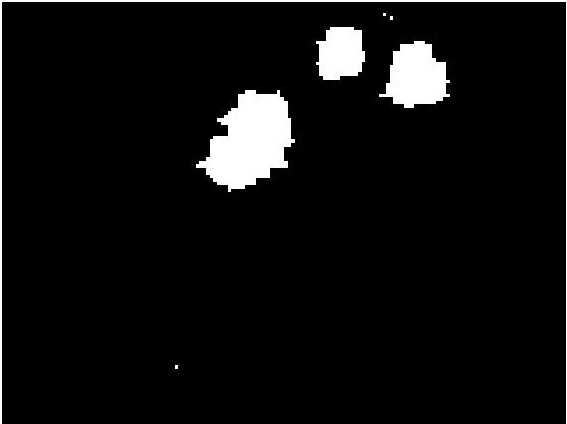
\includegraphics[height=.35\linewidth]{img/fg_morphed.jpg}
    }
    \subfloat[]{
      \label{fig:blobs}
      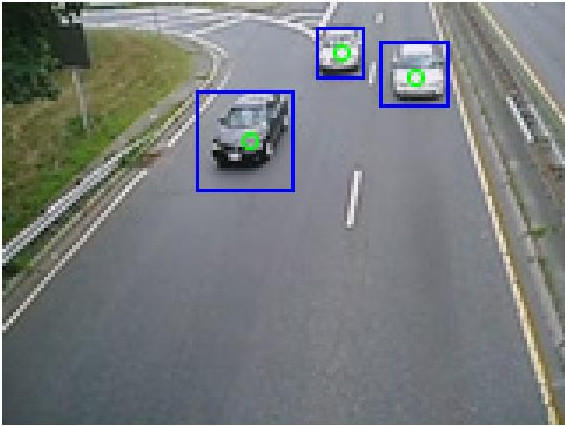
\includegraphics[height=.35\linewidth]{img/blobs.jpg}
    }
  \caption{Steps in the object extraction process. a) shows one frame of the
  video being processed. b) shows the results of applying the mixture of
  Gaussians technique to extract the foreground pixels. c) is the image obtained
after applying dilation, filling and erosion to b). d) shows the centres and
bounding boxes of the extracted blobs.}
  \label{fig:fgextract}
\end{figure}

Once the morphological operations have been applied, we extract information
about the blobs in the image. Blob extraction is done by finding connected
components in an image using 8-connectivity. We use the built in \textsc{Matlab}
algorithm to perform blob extraction. Since we have a thresholded image with
only two colours, either black or white, this operation is relatively simple as
we do not have to define measure of pixel similarity. We receive the centroids
and bounding boxes of the blobs in the image from the algorithm. The blob
detection only returns blobs which have a size larger than 100 pixels, but this
is adjustable depending on the situation in which the system is being used. An
example of overlaying the results onto the original image can be seen in
Figure~\ref{fig:blobs}.
\section{Kalman Filter}
\subsection{Basic Formulation}
The first of the two filtering methods that we used in our implementation is
the Kalman filter. It uses a multivariate Gaussian to represent the state of the
system, and a process model $R$ and measurement model $Q$ to represent the noise
in the system. The basic Kalman filter is a linear estimator, which means that
it assumes that the evolution of the system follows some sort of linear
equations. The extended Kalman filter allows the use of nonlinear equations in
the state evolution. However, in our system we make the assumption that objects
are moving in a linear fashion. This is a reasonable assumption, since in the
vast majority of highway scenes vehicles will be moving in straight lines. 

First, we define the state vector $\mathbf{x}$ of the system as
\begin{equation}
  \label{eq:statevec}
  \mathbf{x}^T=\left[x\;y\;w\;h\;\dot{x}\;\dot{y}\right]
\end{equation}
where $x$ and $y$ are the position of the centre of the object in the image, $w$
and $h$ are the width and height of the bounding box of the object, and
$\dot{x}$ and $\dot{y}$ are the velocities of the object centre in the $x$ and $y$
directions. In our case, the origin is in the top left of the image. We have
included the bounding box dimensions in our state vector as this allows us to
attempt to estimate the change in size of the bounding box as the system
evolves, and to maintain a better estimate of the bounding box even if the
measurement received is not accurate.

Our measurement vector $\mathbf{z}$ is
\begin{equation}
  \label{eq:measvec}
  \mathbf{z}=\left[c_x\;c_y\;b_w\;b_h\right]
\end{equation}
where $(c_x,c_y)$ is the centroid received from the blob detection, and $b_w$ and
$b_h$ are the width and height of the bounding box. The blob detection can extract
several different blobs, so several of these vectors can be received in each timestep.

The Kalman filter process has two major steps; the prediction step and
the update step.  In the prediction step, the next state of the system is
predicted using the previous state and the state transition matrix $A$ and the
process model as follows
\begin{align}
  \bar{\mu}_t&=A\mu_{t-1}+Bu_{t-1}\\
  \bar{\Sigma}_t&=A\Sigma_{t-1}A^T+R
\end{align}
In most systems, there is some control input that is received by the system to
modify its state, but in this case we have no control input, so $B=0$, and that
term is not relevant in the update --- we rely purely on the state transition
model to modify the state. The prediction step computes the predicted
mean~$\bar{\mu}$ and covariance~$\bar{\Sigma}$ for the $t$th timestep. At any
point in time, the value of $\Sigma$ indicates the uncertainty in the system,
and $\mu$ indicates the point around which the Gaussian is centred, that is,
the most probable current state. We have set $A$ as
\begin{equation}
  \label{eq:amat}
  A=\begin{bmatrix}
    1&0&0&0&dt&0\\
    0&1&0&0&0&dt\\
    0&0&1&0&0&0\\
    0&0&0&1&0&0\\
    0&0&0&0&1&0\\
    0&0&0&0&0&1
  \end{bmatrix}
\end{equation}
where $dt$ is the time elapsed between updates. Since we process every frame,
this is generally 1. The process model $R$ is dependent on the particular video
sequence that is being processed, and is of the form
\begin{equation}
  \label{eq:rmat}
  R=\begin{bmatrix}
    \sigma_x^2&0&0&0&0&0\\
    0&\sigma_y^2&0&0&0&0\\
    0&0&\sigma_w^2&0&0&0\\
    0&0&0&\sigma_h^2&0&0\\
    0&0&0&0&\sigma_{\dot{x}}^2&0\\
    0&0&0&0&0&\sigma_{\dot{y}}^2
  \end{bmatrix}
\end{equation}
The measurement model is dependent on the efficacy of the blob detection, and
the quality of the camera, and is of the form
\begin{equation}
  \label{eq:qmat}
  Q=\begin{bmatrix}
    \sigma_{c_x}^2&0&0&0\\
    0&\sigma_{c_y}^2&0&0\\
    0&0&\sigma_{b_w}^2&0\\
    0&0&0&\sigma_{b_h}^2\\
  \end{bmatrix}
\end{equation}
Since multiple measurements may be received, it is necessary to associate the
correct measurement with the filter in order to choose which measurement to use
in the update step. There may be multiple measurements, but we are only
interested in the measurement which is closest to the state of the filter after
the prediction step. Association is done by comparing all measurements obtained
to the mean of the filter and choosing the one with the lowest Mahalanobis
distance. This process can also be used to compute outliers. An observation
model $H$ is defined which allows us to transform the state vector into a form
that can be compared with the measurements. As the measurement and the state
vector contain essentially the same parameters, this matrix is simply
\begin{equation}
  H=
  \begin{bmatrix}
    1&0&0&0&0&0\\
    0&1&0&0&0&0\\
    0&0&1&0&0&0\\
    0&0&0&1&0&0
  \end{bmatrix}
\end{equation}

After incorporating the measurement uncertainty into the uncertainty after the
prediction step, we compute the innovation $\nu$, which is the difference
between the predicted measurement and the one received $\hat{z}_t$. This is then
used to compute the Mahalanobis distance $D$. This is passed into a Gaussian to
compute the probability $\Psi$ of taking that measurement. Outliers are those
measurements for which $D>\lambda_M$, where $\lambda_M$ is a value sampled from
the inverse $\chi^2$ distribution with 4 degrees of freedom, which gives a
boundary on the Mahalanobis distance below which we expect most measurements to
fall \cite{thrun2005prob}. We make the assumption that our measurements are
accurate, and so $\lambda_M=\text{Inv-}\chi^2(0.99,4)$.
\begin{align}
  \label{eq:assoc1}
  S_t&=H\bar{\Sigma}_tH^T+Q\\
  \nu_t&=z_t-H\bar{\mu}_t\\
  D&=\nu_t^TS_t^{-1}\nu_t\\
  \label{eq:assoc4}
  \Psi&=\frac{1}{2\pi \det(S)^{\frac{1}{2}}}\exp^{-\frac{1}{2}D}
\end{align}

The process in Equations~\eqref{eq:assoc1}--\eqref{eq:assoc4} is repeated for
each measurement, and the measurement which corresponds to the maximum value of
$\Psi$ is the one which is used in the measurement update.

Finally, the measurement chosen is incorporated into the filter to update the
belief and obtain the final values of $\mu_t$ and $\Sigma_t$. $\mu_t$ is then
used to represent the state of this object.

\begin{align}
  K_t&=\bar{\Sigma}_tH^TS^{-1}\\
  \mu_t&=\bar{\mu}_t+K_t\nu_t\\
  \Sigma_t&=\bar{\Sigma}_t-K_tH\bar{\Sigma}_t
\end{align}
\subsection{Extension to Multiple Objects}
In order to extend the Kalman filter to track multiple objects, it is necessary
to introduce additional distributions into the model somehow. This could be done
using a mixture of Gaussians, where the posterior is represented by a
multimodal Gaussian distribution \cite{thrun2005prob}, but this is not a good
match for our application as it seems to imply that there is a single object
about whose position we have multiple hypotheses. In actual fact, we have
multiple distinct objects, about which we have a single hypothesis. In that
sense, a multimodal distribution to represent a single object seems to be
unnecessary. As such, we have decided to assign a single Kalman filter to each
object as it is detected.

At each timestep, all existing Kalman filters are updated. Each update results
in the computation of outliers, which give information about measurements which
are far from the expected measurements given the filters that are currently
active. Each of the measurements that is an outlier is considered to be an
object which has appeared onto the scene and that has not yet been assigned a
filter. New filters are initialised with the centroid from one of the outlier
measurements. The initial parameters for each filter are
\begin{align}
  \mu_0&=\left[c_x\; c_y\; 0\; 0\right]\\
  \Sigma_0&=
  \begin{bmatrix}
    5&0&0&0&0&0\\
    0&5&0&0&0&0\\
    0&0&5&0&0&0\\
    0&0&0&5&0&0\\
    0&0&0&0&100&0\\
    0&0&0&0&0&100\\
  \end{bmatrix}
\end{align}
The velocity is not known when the measurement is received, so we assign a high
variance to it in order to accommodate possible velocities. The other
parameters, the centroid and the bounding box parameters are comparatively
accurate, so they are assigned a lower variance.

In addition to creating new filters to track newly detected objects, filters
which were created as a result of spurious measurements or for those objects
which have left the scene are deleted. This is done by keeping a count of the
number of consecutive frames in which the filter was not updated as a result of
unreliable or non-existent measurements corresponding to that filter. Filters
are deleted if they are not updated within 2 frames of the last update.
\section{Particle Filter}
\subsection{Basic Formulation}
The particle filter is another common state estimation method, but it is
fundamentally different from the Kalman filter in the sense that it does not
represent its posterior by a Gaussian approximation, but instead uses a
representative sample from a proposal distribution described by a number $N$ of
particles $p_i^t$. This means that it can easily represent multiple hypothesis
situations, such as those occurring in the problem of localisation. By using
another type of filter for the same task we are able to compare the two
approaches.

Much like the Kalman filter, the particle filter has two stages; a propagation
step in which particles are moved according to the process model and the control
action applied. The second step is the measurement update, in which particles
are assigned weights $w_i^t$ according to their correspondence with received
measurements. After weights are assigned, particles are resampled --- particles
are carried over to the next timestep with a probability proportional to their
weight, with the exact proportion dependent on the resampling scheme used. The
particle filter uses the same state vector and receives the same measurements as
the Kalman filter, shown in equations \eqref{eq:statevec} and
\eqref{eq:measvec}. The position of the object centre is shifted according to
the velocities, while velocities and bounding boxes remain the same. The details
of this stage differ somewhat to the Kalman filter, however. While the Kalman
filter only has a single state vector and covariance matrix for each instance,
the particle filter has a comparatively large number of particles it uses to
represent the posterior. As a result, the state transition must be applied to
each particle, which is a complete representation of a possible state of the
system. Herein lies the main computational difference between the Kalman filter
and particle filter; the particle filter needs to update large numbers of
particles in order to represent its belief state, and as a result computations
are often slower.

Before starting the filter it is necessary to initialise the particles according
to our belief about the system state. It is common to distribute particles
uniformly across the whole operational space. In our case, we have decided to
avoid initialisation until measurements have been received, as if there are no
objects in the image frame there will be nothing to track, and so moving
particles around will be pointless. Each particle is initialised by

\begin{equation}
  p_i^t=
  \begin{bmatrix}
    U_xw_k + x_k\\
    U_yh_k + y_k\\
    w_k\\
    h_k\\
    \dot{x}_i\\
    \dot{y}_i
  \end{bmatrix}
\end{equation}
where $U_x,U_y\sim U(0,1)$ are numbers in the range $[0,1]$ independently
sampled from a uniform distribution, $w_k$ and $h_k$ are the width and height of
the bounding box given by the $k$th measurement, and $(x_k,y_k)$ is the centroid
of that bounding box. $\dot{x}_i,\dot{y}_i\sim\mathcal{N}(0,\sigma_v^2)$ are
numbers drawn from a zero-mean normal distribution with variance
$\sigma_v^2$. This initialises particles uniformly within the bounding box of
each of the $k$ measurements, with normally distributed velocities, which can be
either positive or negative, meaning that objects moving upwards and downwards
through the image can be tracked.

Since multiple measurements may be received at initialisation,
particles are split between different objects according to the proportion of the
total area of all bounding boxes which the bounding box for the object
occupies. The number of particles $n$ assigned to the $k$th measurement is
\begin{equation}
  n_k=N\cdot\frac{w_kh_k}{\sum_{i=1}^bw_ih_i}
\end{equation}
where $b$ is the total number of measurements received. To ensure that large
boxes do not receive a disproportionate number of particles, there is a lower
limit on the number of particles that can be assigned to any given object. This
is set in the initialisation of the filter and depends on the number of objects
that are expected to be visible in any given frame.

To perform the propagation step, each particle is updated using
\begin{equation}
  p_i^{t+1}=p_i^t +
  \begin{bmatrix}
    0&0&0&0&dt&0\\
    0&0&0&0&0&dt\\
    0&0&0&0&0&0\\
    0&0&0&0&0&0\\
    0&0&0&0&0&0\\
    0&0&0&0&0&0
  \end{bmatrix}
  p_i^t + \mathcal{N}R
\end{equation}
where $\mathcal{N}$ is a $6\times 1$ column vector containing zero mean normally
distributed random numbers. $R$ is the process noise matrix, identical to
\eqref{eq:rmat}. The matrix is used to modify the $x$ and $y$ position of the
particle according to the velocities and the time $dt$ which has elapsed from
the previous update, which is usually 1, as we do per-frame updates.

After prediction, particles need to be re-weighted in preparation for
resampling. The re-weighting is done based on the distance of the particle to
its closest measurement. We compare only the position and the size of the
bounding box for each measurement and particle, as we do not know the velocity
of measured objects. To save on computation time we use the city block
distance. Distances are computed between every particle and measurement. A
matrix $\nu$ is constructed which contains the differences between each particle
and its closest measurement in its columns. The weight of each particle is then
computed by
\begin{equation}
  \label{eq:pwt}
  w_i^t=\frac{1}{(2\pi)^2\det(Q)^{\frac{1}{2}}}\exp{\left(-\frac{1}{2}\nu_i^TQ^{-1}\nu_i\right)}
\end{equation}
where $Q$ is the measurement model, identical to \eqref{eq:qmat}, and $\nu_i$ is
the $i$th column of $\nu$. The weights are normalised to ensure that they sum to
1.

Finally, the resampling step is applied. In this step, we select which particles
should carry through to the next timestep based on their weight as a proportion
of the total. We use systematic or low variance sampling which reduces the
likelihood of particle deprivation, which is important when using particle
filters, as deprivation can result in the loss of accurate tracking in
comparison to the simple multinomial sampling. We also considered the use of
stratified sampling, but there appeared to be no improvement in the tracking
performance of the filter if it was used. One issue that could possibly arise is
the particle deprivation in one cluster due to very low weights, as systematic
sampling works through the whole particle cloud, so if the total weight of one
cluster is very low, then it may be the case that these clusters are lost, but
in practice we did not notice such issues.

\subsection{Dealing with New Objects}

While the particle filter is designed in such a way that it deals easily with
multiple hypotheses, in its basic form it does not deal with new objects. The
filter does not place any particles in regions where particles are not already
present. This means that even if a new object was to appear and a measurement
for it was received, if there are no particles in that region, then the object
will go ``unnoticed'' by the filter. Thus, we need some method of introducing
particles into these regions in such a way that allows the consideration of new
objects.

A standard technique in many particle filter implementations which attempts to
mitigate the effects of particle deprivation is to add some small proportion of
particles into the scene at random. This gives the filter a chance of creating
new particle clusters in areas of interest that were previously devoid of
particles. This method is not robust enough, however. In order to reliably catch
all new objects entering the scene a large proportion of the total number of
particles would have to be assigned to this randomly reinitialised group. This
would reduce the accuracy of the filter in places where there was an object of
interest, and also wastes computation time and particles on regions of the space
which are completely uninteresting.

In \cite{meier1999tracking}, Meier and Ade propose an extension to the particle
filter which allows it to include new objects in the tracking. This extension
ensures that regions in which measurements appear are populated with some
particles, which allows the tracking of the object if measurements of it
continue to be made.

The first modification is the addition of an initialisation step to the
filter. Usually, the initialisation step is done once, at the beginning of
tracking. In this case, however, a portion of particles are re-initialised at
the beginning of each step of the filter. Taking some $M$ particles, we
initialise them directly on measurements that were received in the previous
timestep. The other particles are the $N-M$ particles which were selected from
the resampling step. This direct initialisation allows new any new objects to be
added to the tracking. If the previous timestep has no measurements, then all
$N$ particles are initialised based on the measurements, as in the first
timestep. When initialising on top of measurements, we considered initialising
particles only on those measurements which were new, that is, those measurements
for which there were no corresponding clusters, but tests indicated that this
led to some particle deprivation issues on existing clusters.

The propagation step is done as usual. When this step is completed,
some of the $M$ particles which were initialised around measurements
corresponding to new objects are likely to have moved into a region close to
that in which the measurement in the current timestep has been received.

A suggestion is also made to weight particles according to
\begin{align}
  w_i^t&=\left\{
      \begin{array}{l l}
        e^{-\frac{1}{2\sigma^2}u^2}&u<\delta\\
        \rho &\text{otherwise}
      \end{array}\\
      u&=\min_k\mid p_i^t-z_m^t\mid
\end{align}
in order to allow those objects which are missing a measurement in a timestep to
continue on to the next and allow continued tracking. However, in our testing of
this weighting scheme, we noticed that it resulted in a large degradation in
performance due to a resulting high spread of particles over the space, and the
difficulty of extracting reliable clusters from which to extract tracking
information. As a result, we have kept the original weighting procedure detailed
in \eqref{eq:pwt}.

The final change required is to modify the resampling step. In the standard
formulation, $N$ particles are chosen based on weight to replace the $N$
particles in the previous step. However, we instead resample only $N-M$
particles. This still results in a fair representation of the posterior, but
allows for the addition of the $M$ particles which are randomly initialised at
the measurement positions at the start of the next timestep.

\section{Results}

\begin{figure}
  \centering
  \subfloat[Frame 65]{
    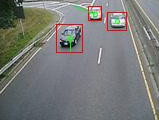
\includegraphics[width=0.4\linewidth]{img/vip_65_pf}
    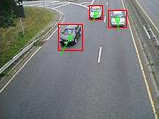
\includegraphics[width=0.4\linewidth]{img/vip_65_kf}
  }\\
  \subfloat[Frame 70]{
    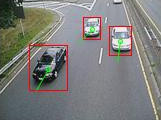
\includegraphics[width=0.4\linewidth]{img/vip_70_pf}
    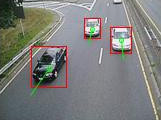
\includegraphics[width=0.4\linewidth]{img/vip_70_kf}
  }
  \caption{Tracking results 5 frames apart, using the particle filter with 10000
    particles (left), and Kalman filter (right). The green velocity vector is
    exaggerated and not adjusted for perspective.}
  \label{fig:viptraf}
\end{figure}

To evaluate the performance of the two filters, we used video from various
sources\footnote{Datasets from http://www.ee.cuhk.edu.hk/\textasciitilde
  xgwang/MITtraffic.html, http://www.edmontontrafficcam.com, and \textsc{Matlab}
  computer vision toolbox.}. Due to the lack of ground truth, it was not
possible to perform a quantitative analysis of the performance, but by looking
at various situations we were able to perform a qualitative analysis.

Figure~\ref{fig:viptraf} shows an example of the output of the two filters. The
particle filter has some issues with regard to the variance of the velocity
vector tracking, which can be seen in one of the images. This is most likely in
part due to the addition of random particles to all clouds, which introduces
some error into the vector. When given enough time the filter generally
fluctuates around the correct vector, but it is not as accurate as is
desirable. The Kalman filter on the other hand, as can be seen from the images
is very consistent in its estimates of the velocity. Both of the filters have
little problem tracking the vehicle centroid.

\begin{figure}
  \centering
  \subfloat[Dark scenes]{
    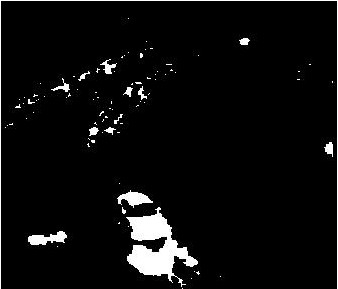
\includegraphics[width=0.4\linewidth]{img/headlight_bg}
    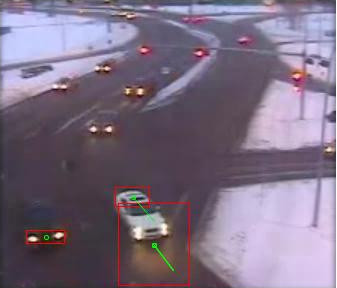
\includegraphics[width=0.4\linewidth]{img/headlight_track}
  }\\
  \subfloat[Occluding vehicles]{
    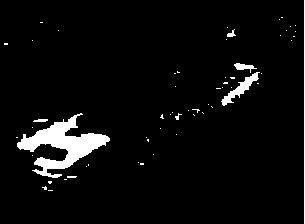
\includegraphics[width=0.4\linewidth]{img/multiblob_bg}
    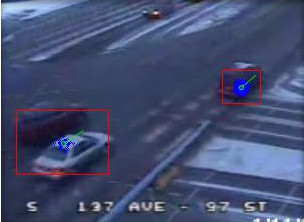
\includegraphics[width=0.4\linewidth]{img/multiblob_track}
  }\\
  \subfloat[Minimum blob too small]{
    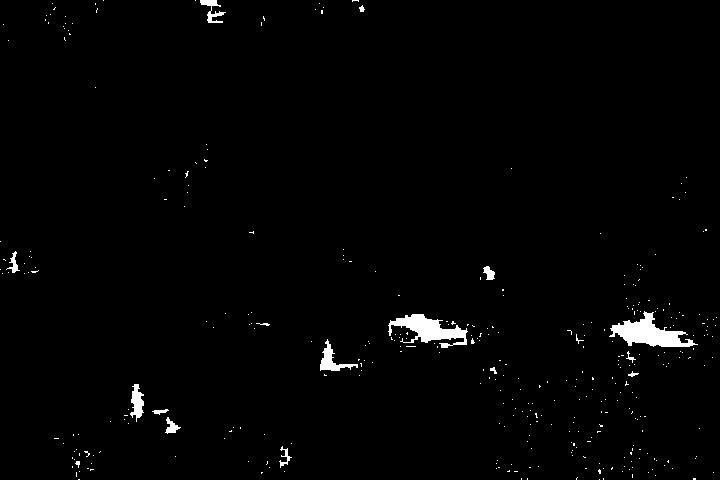
\includegraphics[width=0.4\linewidth]{img/pedestrian_fg}
    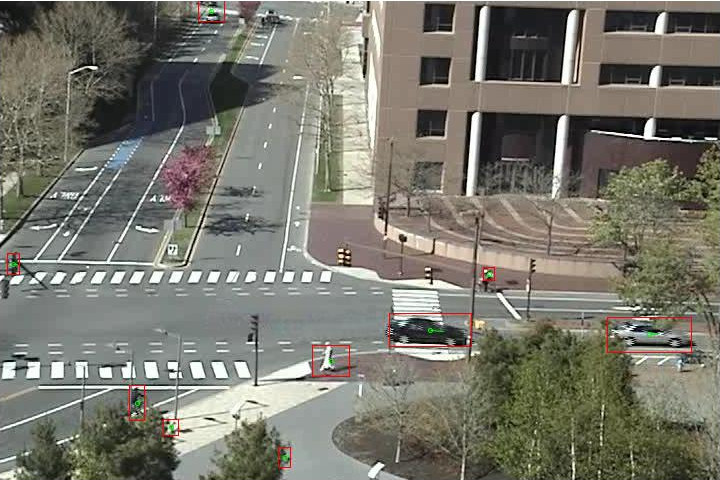
\includegraphics[width=0.4\linewidth]{img/pedestrian_track}
  }
  
  \caption{Causes of filter issues. a) shows some of the problems of dark
    scenes. The vehicle in the bottom centre is treated as two blobs, and one of
    these has its centroid in between its headlights and car itself. In the
    bottom left there is a vehicle which is only visible by its headlights. b)
    shows the effect of two vehicles close to each other on blob detection ---
    they are detected as a single blob, which leads the tracking to see both
    vehicles as only a single one. c) shows the result of a minimum blob size
    which is too low. The filters also track pedestrians.}
  \label{fig:blobissue}
\end{figure}

Many of the problems encountered are a result of the difficulty of getting good
measurements from the blob extraction. In night scenes, the background and
foreground have very similar colours, and headlights cause significant
problems. In scenes with a large number of vehicles which occlude each other,
some blobs end up covering two or more cars. Sometimes two blobs may represent
the same vehicle, and this reduces the accuracy as well. these problems account
for the vast majority of tracking losses. In these difficult scenes, both
filters are still able to detect some vehicles, but the accuracy of both the
Kalman filter and particle filter are significantly reduced. Specifying a
minimum blob size results in the tracking of unwanted objects, some of them
objects which might be useful to track, such as people or cyclists, but it also
results in the tracking of spurious blobs. Figure~\ref{fig:blobissue} shows some
of these issues.

Average processing time on one run of $160\times 120$ pixel video with Kalman
filter is 0.215 frames/sec, compared to 0.487 frames/sec for the particle filter
with 10000 particles. The timing includes foreground and blob extraction, filter
processing and then image display. 


\section{Conclusion}
In this report, we have presented a system for the tracking of multiple vehicles in a highway
environment using augmented versions of the Kalman filter and particle
filter. Video frames are separated into foreground and background pixels using a
mixture of Gaussians. Foreground pixels are processed using morphological
operations and then a blob detection algorithm is run to extract the centroid
and bounding box of the blob. This information is used by the filters to track
different objects in the image.

The system is able to process videos of approximately $160\times 120$ pixels at
a rate of 5 frames/sec with the Kalman filter, and 2 frames/sec with the
particle filter using 10000 particles, on an Intel i7-3520M at 2.9 GHz. This
includes application of mixture of Gaussians, blob extraction, morphological
operations and insertion of bounding boxes and centres into the image. As we had
no ground truth, it was not possible to do a quantitative investigation of the
errors, but qualitative investigation indicates that the Kalman filter is
generally very accurate, whereas the particle filter suffers from some issues
with regards to the velocity of vehicles, which has a high variance.

There are numerous ways in which the system could be improved. First, improved
blob extraction and a more reliable mixture of Gaussians could result in better
measurements being received by the filters. Reduction of blob merging and issues
with shadows could be done by applying the lane dividing technique suggested in
\cite{hsieh2006automatic}. Initial velocity estimates for objects could be
improved using a-priori road information, as suggested by
\cite{magee2004tracking}.

\printbibliography

\end{document}
